%
% File acl2021.tex
%
%% Based on the style files for EMNLP 2020, which were
%% Based on the style files for ACL 2020, which were
%% Based on the style files for ACL 2018, NAACL 2018/19, which were
%% Based on the style files for ACL-2015, with some improvements
%%  taken from the NAACL-2016 style
%% Based on the style files for ACL-2014, which were, in turn,
%% based on ACL-2013, ACL-2012, ACL-2011, ACL-2010, ACL-IJCNLP-2009,
%% EACL-2009, IJCNLP-2008...
%% Based on the style files for EACL 2006 by 
%%e.agirre@ehu.es or Sergi.Balari@uab.es
%% and that of ACL 08 by Joakim Nivre and Noah Smith

\documentclass[11pt,a4paper]{article}
\usepackage[hyperref]{acl2021}
\usepackage[utf8]{inputenc}
%\usepackage[T1]{fontenc}
%\usepackage[encoding]{fontenc}
\usepackage{times}
\usepackage{latexsym}
\renewcommand{\UrlFont}{\ttfamily\small}
\usepackage{amsmath,amsfonts,amssymb}
\usepackage[noabbrev,capitalize]{cleveref}
\usepackage{xargs}
\usepackage{graphicx}
%\usepackage[colorinlistoftodos,prependcaption,textsize=tiny]{todonotes}
%\newcommandx{\jp}[2][1=]{\todo[linecolor=purple,backgroundcolor=purple!25,bordercolor=purple,#1]{#2}}

% This is not strictly necessary, and may be commented out,
% but it will improve the layout of the manuscript,
% and will typically save some space.
\usepackage{microtype}

\usepackage{pgfplots}
\usepackage{pgfplotstable}
    \pgfplotsset{
        compat=1.9,
        compat/bar nodes=1.8,
    }
    \pgfplotstableread{
        lang natural hallucinated
        tur	100310 0
        olo	100062 0
        vep	100053 0
        sah	100046 0
        por	100041 0
        pol	100039 0
        ara	100027 0
        tyv	100015 0
        kmr	100003 0
        rus	100002 0
        spa	100001 0
        aym	100000 0
        deu	100000 0
        ces	94169 0
        krl	78673 0
        bul	39011 0
        nld	38827 0
        amh	32254 0
        heb	23204 0
        afb	22165 0
        arz	17683 0
        cni	13948 0
        ckb	11577 0
        ind	11072 0
        evn	5216 10000
        see	3801 10000
        ame	2524 10000
        itl	1246 10000
        syc	1217 10000
        bra	1082 10000
        ail	918 10000
        mag	854 10000
        vro	804 10000
        kod	323 10000
        sjo	290 10000
        gup	214 10000
        ckt	132 10000
        lud	128 10000
    }\testdata

%\aclfinalcopy % Uncomment this line for the final submission
%\def\aclpaperid{***} %  Enter the acl Paper ID here

%\setlength\titlebox{5cm}
% You can expand the titlebox if you need extra space
% to show all the authors. Please do not make the titlebox
% smaller than 5cm (the original size); we will check this
% in the camera-ready version and ask you to change it back.

\newcommand\BibTeX{B\textsc{ib}\TeX}

\title{Training Strategies for Neural Multilingual Morphological Inflection}

\author{First Author \\
  Affiliation / Address line 1 \\
  Affiliation / Address line 2 \\
  Affiliation / Address line 3 \\
  \texttt{email@domain} \\\And
  Second Author \\
  Affiliation / Address line 1 \\
  Affiliation / Address line 2 \\
  Affiliation / Address line 3 \\
  \texttt{email@domain} \\}

\date{}

\begin{document}
\maketitle
\begin{abstract}
something something something something something something
something something something something something something
something something something something something something
something something something something something something
something something something something something something
something something something something something something
something something something 
\end{abstract}

\section{Introduction}

Morphological inflection is the task of transforming a lemma to its
inflected form given a set of grammatical features. 
The task requires a model to recognize which morphological processes
should be applied to the word, such as affixing, circumfixing and
reduplication, among others. 

The worlds languages exhibit a large variety of strategies. In
addition to the morphological processes, languages use different
strategies to encode the grammatical features. Typically, languages
fall into a spectrum ranging from agglutinative to isolating. In
agglutinative languages grammatical features are encoded with
morphemes attached to a lemma, while in isolating languages each
grammatical feature is repersented as a lemma.

Several systems for inflecting words have been implemented both using
statistial and rule-bsed methods. In rule-based methods rules for
transformatins of strings are identified and applied accordingly. In
this paper we focus on morphological inflection with neural networks,
specifically, multilingual systems. In a multilingual system, a single
model is developed to process multiple languages, such that we can
give it either a word in for example Swedish or Evenk that will be
inflected.

This is a challenging problem as language recources for many languages
is scarce, so a multilingual system must be able to model inflectional
processes given varying amounts of data. In this paper we mainly focus
on \emph{training strategies} for multilingual systems. That is, given
a baseline system, which augmentations to the training schema help a
model to produce ...


%In this paper we explore different training schemas for neural
%networks, in a multilingual model for morphological inflection in 37
%different languages.

%We are particularly interested in how far we can get using a simple
%LSTM sequence-to-sequence model with attention, augmented with
%training procedures informed by human heuristics.

We employ a LSTM encoder-decoder architecture with attention as our
base model and consider the following training strategies:

\begin{itemize}
\item Curriculum learning: We augment the order in which the examples are presented to the model based on the loss.
\item Multi-task learning: We predict the formal operations required to transform a lemma into its inflected form.
\item Language-wise label smooothing: We smooth the loss function to not penalize the model as much when it predicts a character from the correct language.
\item Scheduled sampling: We use a probability distribution to determine whether to use the previous output or the gold as input when decoding.
\end{itemize}

\section{Task}

As mentioned previously the task of morphological inflection is to
predict the \emph{inflectional form} of a lemma (the ``base'' form of
a word) given a set of grammatical features (such as \texttt{tense} or
\texttt{person}).
%
%- tag
%- lemma
%- prediction (inflected form)

%[perhaps: Describe edition tasks here as well (as auxiliary tasks)]

\section{Data}

The data released cover $37$ languages of varying typology, geneology,
grammatical featues and morphological processes. The data for the
different languges vary greatly in size, from $138$ examples (Ludic) to
$100310$ (Turkish) presenting a unique challange to multilingual
systems.

For the low-resourced languages we produce \textbf{hallucinated data}
to train on. We follow [REF], and produce an inflected form by
replacing the parts of a inflected form which overlap with the lemma.

\begin{figure}
\centering
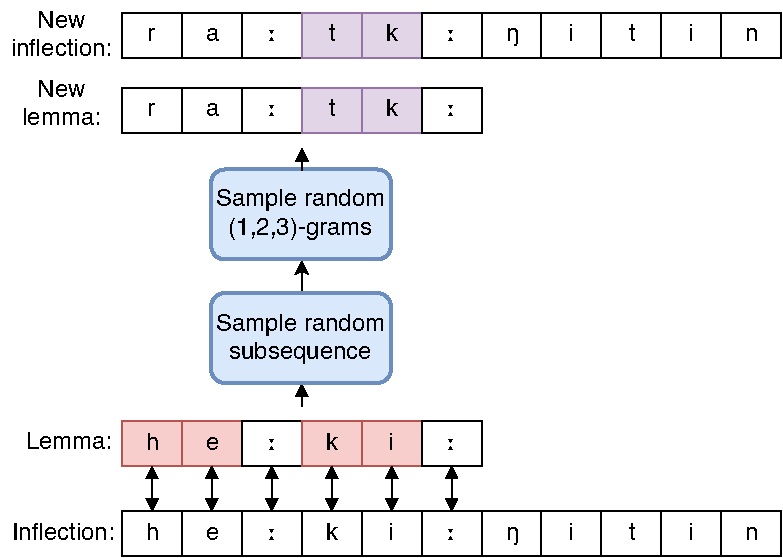
\includegraphics[scale=0.5]{hall.pdf}
\caption{A example of the data hallucination process.}
\end{figure}

We make several additions, when replacing a sequence of characters we
consider combinations of $[1,2,3,4]$-grams. We allow for the
replacement sequence to vary in size, potentially adding or removing 2
characters. Additionally, we don't consider subsequences which include
a phonological symbol.  For each language with fewer than 10 000
examples, we sample 10 000 new examples. A visualization of the number
of examples in each language is shown in

\begin{figure}[ht]
\begin{tikzpicture}
    \begin{axis}[
        ybar stacked,
        ymin=0,
        ymax=105000,
        xtick=data,
        legend style={
            cells={anchor=west},
            legend pos=north east,
        },
        width=\columnwidth*1.15,
        height=150pt,
        /pgf/bar width=4pt,
        reverse legend=true,
        %xtick={100, 1000, 10000, 100000},
        xticklabels from table={\testdata}{lang},
        xticklabel style={text width=1cm,align=center,font=\tiny,rotate=90},
        yticklabel style={text width=1cm,align=center,font=\tiny,rotate=90}
        %x tick label style={rotate=180,anchor=east},
        %xticklabel style = {font=\tiny,yshift=0.5ex}
    ]
        \addplot [fill=green!50]
            table [y=natural, meta=lang, x expr=\coordindex]
                {\testdata};
                    \addlegendentry{natural}
        \addplot [fill=blue!50]
            table [y=hallucinated, meta=lang, x expr=\coordindex]
                {\testdata};
                    \addlegendentry{hallucinated}
    \end{axis}
\end{tikzpicture}
\caption{\label{fig:data} Number of natural and hallucinated examples in each language.}
\end{figure}

We improve upon [REF] in the following way.
Noting that certain languages in the data use phonological symbols
and separators, we hallucinate in such a way that we don't break apart
morphemes.%\jp{An example will help.}


\section{Method}

In this section the multilingual model and training strategies used
are presented. We employ a single model with shared parmeters
across all languages. 

\subsection{Model}

We employ a encoder-decoder architecture with attention. The first
layer in the model is comprised of an LSTM, which produces a
contextual representation for each character in the lemma.

We encode the tags using a self-attention module (equivalent to a
1-head transformer layer).  This layer does not use any positional
data: indeed the order of the tags does not matter.

We use an LSTM decoder with two attention modules. One attending to
the lemma and one to the tags. For the lemma attention we use a
content-based attention module which uses cosine similarity (called
Cosim by [REF]).  However, we found that using Cosim attention only
causes attention to be too focused on a single character, and mostly
ignored contextual cues relevant for the generation.

To remedy this, we combine the cosine attention with additive
attention as follows, where superscript $cos$ indicate cosine attention,
$add$ additive attention and $k$ the key:
%\jp{
%  1. Double-check the code.
%  2. Use another naming than additive (I think it's multiplicative)}

\begin{align*}
	a^{add} & = \mathsf{softmax}(w^\top\mathsf{tanh}(W_ak + W_bh))\\
	att^{add} & = \sum_{t=1}^{T}a_t^{add}h_t^{add}\\
	a^{cos} & = \mathsf{softabs}(cos(k,h))\\
	att^{cos} & = \sum_{t=1}^{T}a_t^{cos}h_t^{cos}\\
	att & = W[att^{cos}; att^{add}]
\end{align*}
(in the above $h_t$ refers to the encoder's contextual representation for each character.)
We employ additive attention for the tags. In each step we pass the
concatenation of the character embedding obtained from the previous
step, the lemma attention and the tag attention to the decoder.

% \[\text{input}_t = [e_{t-1}; att_{char}; att_{tag}]\]

\subsection{Multi-task learning}

Instead of predicting the inflected form, one can also predict the
levenshtein operations needed to transform the lemma into the
inflected form [REF].

We find that making \emph{both} predictions, as a multitask setup,
improves the performance of the system.

The multi-task setup operates on the character level, thus for each
contextual representation of a character we want to predict an
operation. Because \texttt{add} and \texttt{del} change the length, we
predict two sets of operations, the \textbf{lemma-reductions} and the
\textbf{lemma-additions}.

%We break down the task of applying levenshtein-distance operations
%into two sub-tasks: \textbf{lemma-reductions}, where we predict the copy and
%deletion operations and \textbf{lemma-additions}, where we predict the copy and
%addition operations. 

\begin{figure}[ht]
\centering
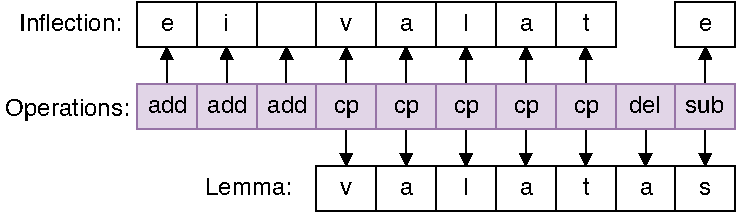
\includegraphics[scale=0.5]{ops.pdf}
\caption{Levenshtein operations mapped to characters in the lemma and inflection.}
\end{figure}

To predict the operations, we pass the lemma representations from the
encoder and the generated inflection representations to a single operation
classification layer.

%For each sub-task we predict the operation based on the hidden states
%generated by our neural network. In the case of lemma-reductions we
%predict the operation on the hidden-states of the encoded lemma. For
%lemma-additions, we predict the operations on the generated characters
%from the decoder.

\subsection{Curriculum Learning}

We use the easy-first curriculum strategy [REF] to sort the data after
each epoch. For all examples in the batch we sort them according to
the loss obtained in the previous epoch, in ascending order such that
the easy (low loss) occurs before the difficult examples (high loss).

For the first epoch, when we dont have any loss to sort by, we sort
the dataset according to the ratio of copy operations to other
operations. We found that this strategy performed better than any of
the other strategies which we tested: fewest addition-operations,
least-grammatical-features, and random.
This strategy causes a small, but consistent improvement in the loss
of the first epoch, which persists throughout the learning process.

\subsection{Scheduled Sampling}

Commonly when training a encoder-decoder model the gold is used as input at
time-step $t$, not the output from the decodet at $t-1$.
It has been shown that models trained with this strategy may suffer
at inference time. Indeed, they have never been exposed to a partially
incorrect input in the training phase.  To address this issue we use
scheduled sampling [REF].

We implement a simple schedule for calculating the probability of
using the gold characters or the model's prediction by using a global
sample-probability variable which is updated at each epoch. We start
with a probability \(\rho\) of 100\% to take the gold. At each epoch
we decrease it by 4\%. For each character, we take sample from the
Bernoulli distribution of parameter \(\rho\) to determine the
decision to make.

\subsection{Training}

We use cross-entropy loss for the character generation loss and 
%We use KL-divergence loss for the characters
%\jp{But the entropy of the
%  label distribution is constant? So this is a red flag. If it's a
%  workaround for a bug in pytorch, this should come down to a
%  footnote.} 
%and cross-entropy loss 
for the operation predictions tasks. Our final loss function consists
of the character generation loss, the lemma-reduction and the
lemma-addition losses summed.

\paragraph{Language-wise Label smoothing} We use language-wise label
smoothing to calculate the loss. This means that we remove $\alpha$
from the probability of the correct character and distribute the same
$\alpha$ uniformly across the probabilities of the characters
belonging to the language of the word. However, each language
potentially uses a different set of characters. We calculate this set
using the the training set only--- so it is important to make $\alpha$
not too large, so that the model does not completely exclude unseen
characters from its prediction at test-time. (We found that
\(\alpha=2.5\%\) is a good value.)

\paragraph{Learning rate decay with a Curriculum} The training
examples will be sorted by the difficulty in the previous epoch.  We
note that employing a decaying learning rate has the effect that a
model update its parameters \textit{more} on the easy examples and
less on difficult examples. The idea is that the morphological
processes involved in more difficult words can be discovered from the
operations involved in the easier examples.

The hyperparameters used for training are presented in \cref{tab:hp} below.
\begin{table}[h]	
\centering
\begin{tabular}{lc}
\textsc{Hyperparameter} & \textsc{Value} \\
  \hline
  Batch Size & 256 \\
  Embedding dim & 128 \\
  Hidden dim & 256 \\
  Epochs & 30 \\
  Initial LR & 0.001 \\
  Min LR & 0.0000001 \\
  Smoothing-$\alpha$ & 2.5\% \\
\end{tabular} 
\caption{Hyperparameters.}
\label{tab:hp}
\end{table}

\section{Results}

\begin{table}[h]	
\centering
\begin{tabular}{lc}
\textsc{Language} & \textsc{Accuracy} \\
  \hline
  
\end{tabular} 
\caption{Acc}
\label{tab:accuracy}
\end{table}



\subsection{Ablation Study}

We perform a leave-one-out ablation study to estimate the effect of
our training strategies. The we use the same hyperparameters as
reported in TABLE, but train for 15 epochs.


%\jp{Not sure if ablation is the right word here.}

\begin{table}[h]	
\centering
\begin{tabular}{lll}
\textsc{Module} & \textsc{Accuracy} & \textsc{EM} \\
  \hline
  All  & $76.6$ & $95.5$ \\
  w/o Multitask & $75.7 (-0.9)$ & $95.0$ \\
  w/o Scheduled sampling & $75.3 (-1.3)$ & $95.1$ \\
  w/o Label smoothing & $74.1 (-2.5)$ & $93.3$ \\
  w/o Curriculum learning & $77.2 (+0.6)$ & $95.7$ \\
\end{tabular} 
\caption{Ablation study.}
\label{tab:abl}
\end{table}

\section{Discussion}

In this paper we focus on training strategies rather than
architectural design. An advantage of finding good training strategies
is that they do not require any additional parameters in the
model. This allows a model to obtain better representations with fewer
parameters, thus increasing the quality of representations without
needing additional encoding parameters.  

\section{Conclusions}


%\section*{Acknowledgments}

%The acknowledgments should go immediately before the references. Do not number the acknowledgments section.
%\textbf{Do not include this section when submitting your paper for review.}

\bibliographystyle{acl_natbib}
\bibliography{acl2021}

%\appendix



\end{document}
